W pracy założono, że pojazdy rolnicze w przybliżeniu są bryłami sztywnymi.
Obiekty te charakteryzują się w przestrzeni trójwymiarowej sześcioma stopniami swobody.
Jednym ze sposobów matematycznego opisu położenia tychże pojazdów w przestrzeni trójwymiarowej,
jest podanie współrzędnych środka ciężkości (x,y,z) oraz trzech parametrów kątowych: azymutu, odchylenia od poziomu w płaszczyźnie poprzecznej oraz podłużnej.
W dalszej części rozdziału opisano kilka przykładowych rozwiązań algorytmów sterowania,które charakterytzują się różnym podejściem 
w odniesieniu do parametrów kątowych określania orientacji przestrzennej pojazdów rolniczych. 
\section{Podział algorytmów sterowania ze względu na dostarczane dane wejściowe}
Jednym z najbardziej popularnych zbiorów parametrów nawigacyjnych, które są następnie wysyłane do algorytmów sterowania, jest para:
azymut plus offset obliczane względem zadanej trasy. Azymut jest to kąt którego ramionami są:
główna oś symetrii pojazdu oraz styczna do krzywej prowadzenia w punkcie, który stanowi rzut prostopadły środka ciężkości na tą krzywą.
Offset natomiast jest to odległość środka ciężkości pojazdu względem zadanej ścieżki \cite{CCTA_769_775}.
Na rysunku nr \ref{fig:ch3_azymutOffset} przedstawione są powyższe parametry. Środek ciężkości pojazdu oznaczono jako C,
azymut pojazdu względem zadanej źcieżki oznaczono jako $\psi$. $\delta$ oznacza kąt sterujący jako wynik przetwarzania algorytmu sterującego tzw. Target Angle.    
\begin{figure}[H] 
\centering
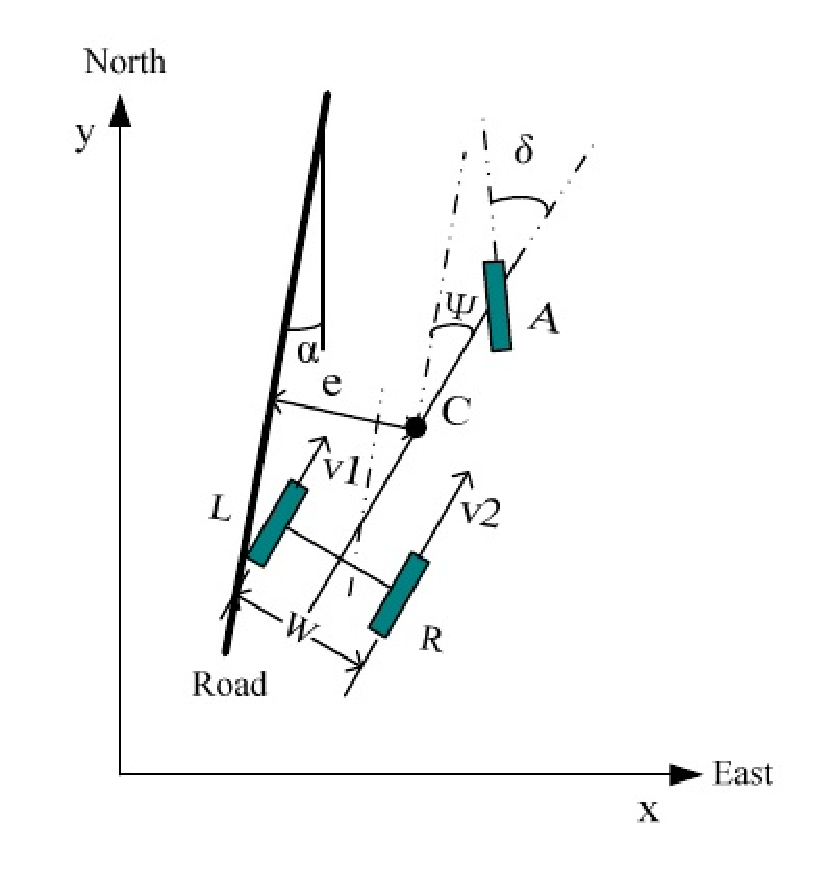
\includegraphics[scale=0.5]{ch3_azymutOffset.eps}
\caption{\textit{Azymut oraz offset - Parametry najczęściej używane w celu wyznaczenia pozycji względem zadanej trasy;}
źródło: \cite[][strona 464]{CCTA5_461_469}}
\label{fig:ch3_azymutOffset}
\end{figure}

W przypadku niskiej dokładności parametrów nawigacyjnych autorzy publikacji \cite{CCTA_943_950}
zaproponowali algorytm, który korzysta tylko z obliczanego w czasie rzeczywistym offsetu.
\begin{figure}[H]
\centering
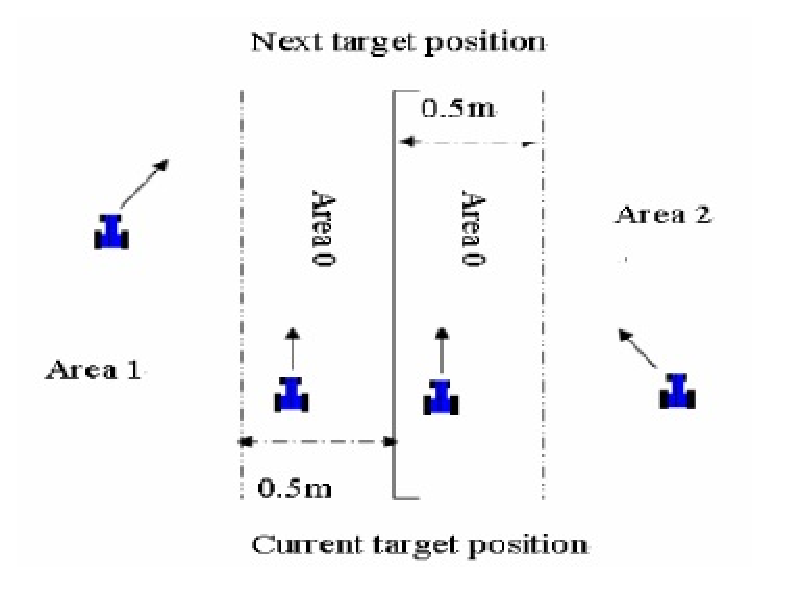
\includegraphics[scale=0.8]{ch3_currentNextTargetPosition.eps}
\caption{\textit{Tylko offset - w przypadku niskiej jakości danych wejściowych;} 
	źródło: \cite[][strona 947]{CCTA_943_950}}
\label{fig:ch3_currentNextTargetPosition}
\end{figure}

\section{Podział algorytmów sterowania ze względu na zastosowane algorytmy decyzyjne}
Różnego rodzaju algorytmy sterowania są używane w celu kompencacji zmiennej dynamiki pojazdów oraz w celu osiągnięcia satysfakcjonującej wydajności sterowania
 \cite[][strona 770]{CCTA_769_775}. Poniżej znajdują się przykłady kilku najbardziej popularnych algorytmów prowadzenia pojazdów:
feedforward plus PID steering control algorithm
